Блок-схема установки изображена на рисунке \ref{fig:exp_setup}.\par
\begin{figure}[ht]
    \centering
    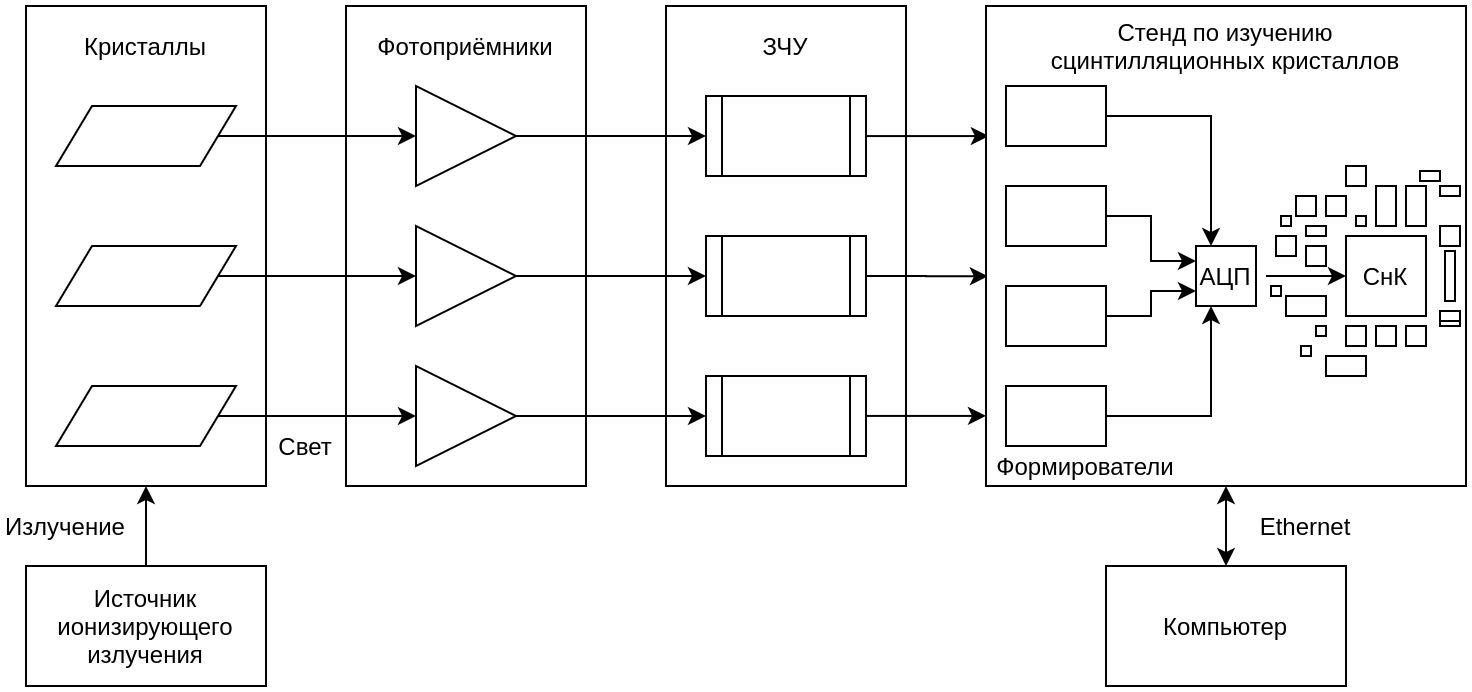
\includegraphics[width=1\linewidth]{Experimental_setup.png}
    \caption{Блок-схема установки}
    \label{fig:exp_setup}
\end{figure}
Ионизирующее излучение с источника попадает на три сцинтилляционных кристалла: исследуемый и два вспомогательных. Излучаемые кристаллами фотоны регистрируются в фотоприёмниках и преобразуются в электрические сигналы. После усиления в ЗЧУ сигналы подаются на входные каналы стенда, где они обрабатываются. Результат обработки отправляется на компьютер оператора через интерфейс Ethernet. Стенд имеет, кроме основного канала, предназначенного для исследуемого кристалла, два дополнительных --- для вспомогательных кристаллов.\par
Стенд является ключевым элементом установки. На рисунке \ref{fig:board_scheme} представлена его блок-схема.\par
\begin{figure}[ht]
    \centering
    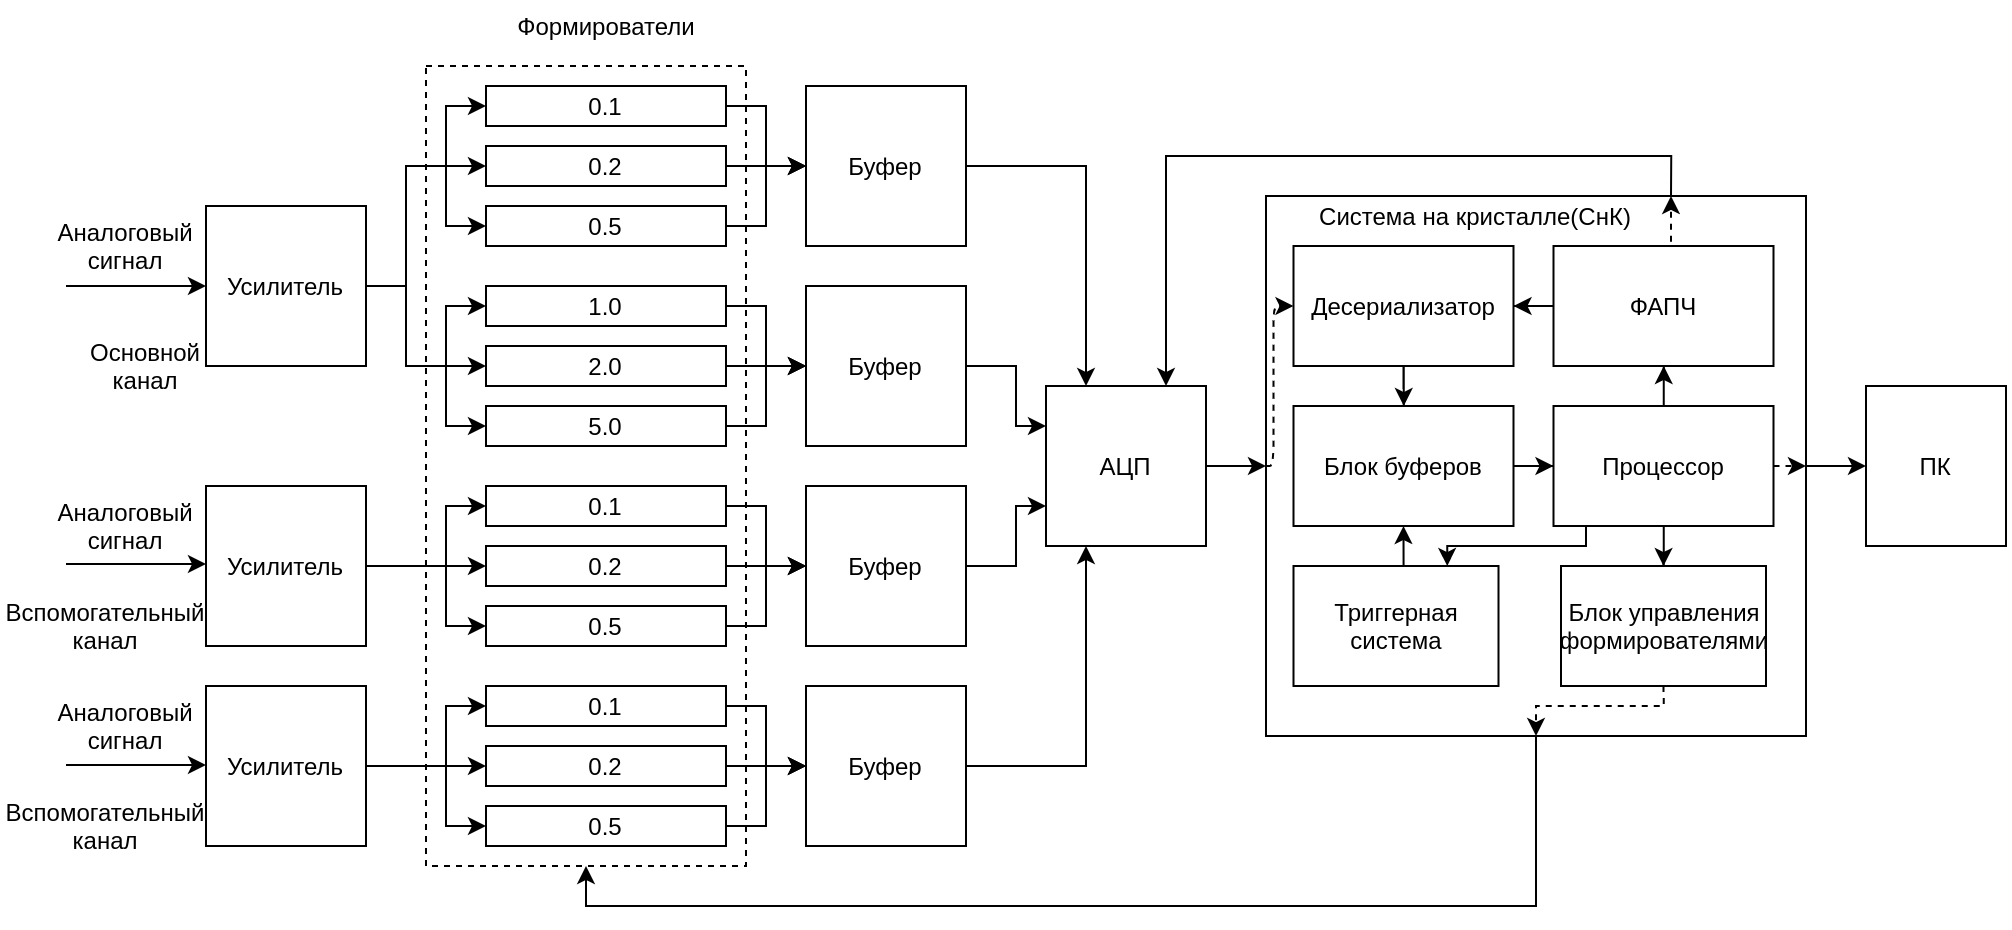
\includegraphics[width=1\linewidth]{board_scheme.png}
    \caption{Блок-схема стенда}
    \label{fig:board_scheme}
\end{figure}
Стенд имеет 3 входных канала: основной и 2 вспомогательных. На каждом из них предусмотрен усилитель, сигнал с которого передаётся в набор формирователей, определяющих время формирования. Далее через промежуточный буфер с дифференциальным выходом сигнал поступает в 14-битный АЦП, где производится его конвертация в цифровой вид. Оцифровка происходит на тактовой частоте 100 МГц, выдаваемой модулем фазовой автоподстройки частоты (ФАПЧ), реализованным в системе на кристалле. Цифровые данные в последовательно упакованном формате передаются в СнК, где проводится их обработка.\par
В первую очередь, происходит обратная конвертация из последовательности бит в число (десериализация), после чего, при срабатывании триггерной системы, данные из блока буферов отправляются в процессор для последующей обработки. Для связи с компьютером используется протокол Ethernet.\par
На рисунке \ref{fig:board} представлена фотография стенда с выделением основных блоков:\par
\begin{enumerate}
    \item Блок питаний;
    \item Система на кристалле Zynq-7000 с необходимой периферией;
    \item 4-х канальный АЦП;
    \item Формирователи основного и вспомогательных каналов;
    \item Усилители сигналов;
    \item Входные разъёмы. 
\end{enumerate}

\begin{figure}[ht]
    \centering
    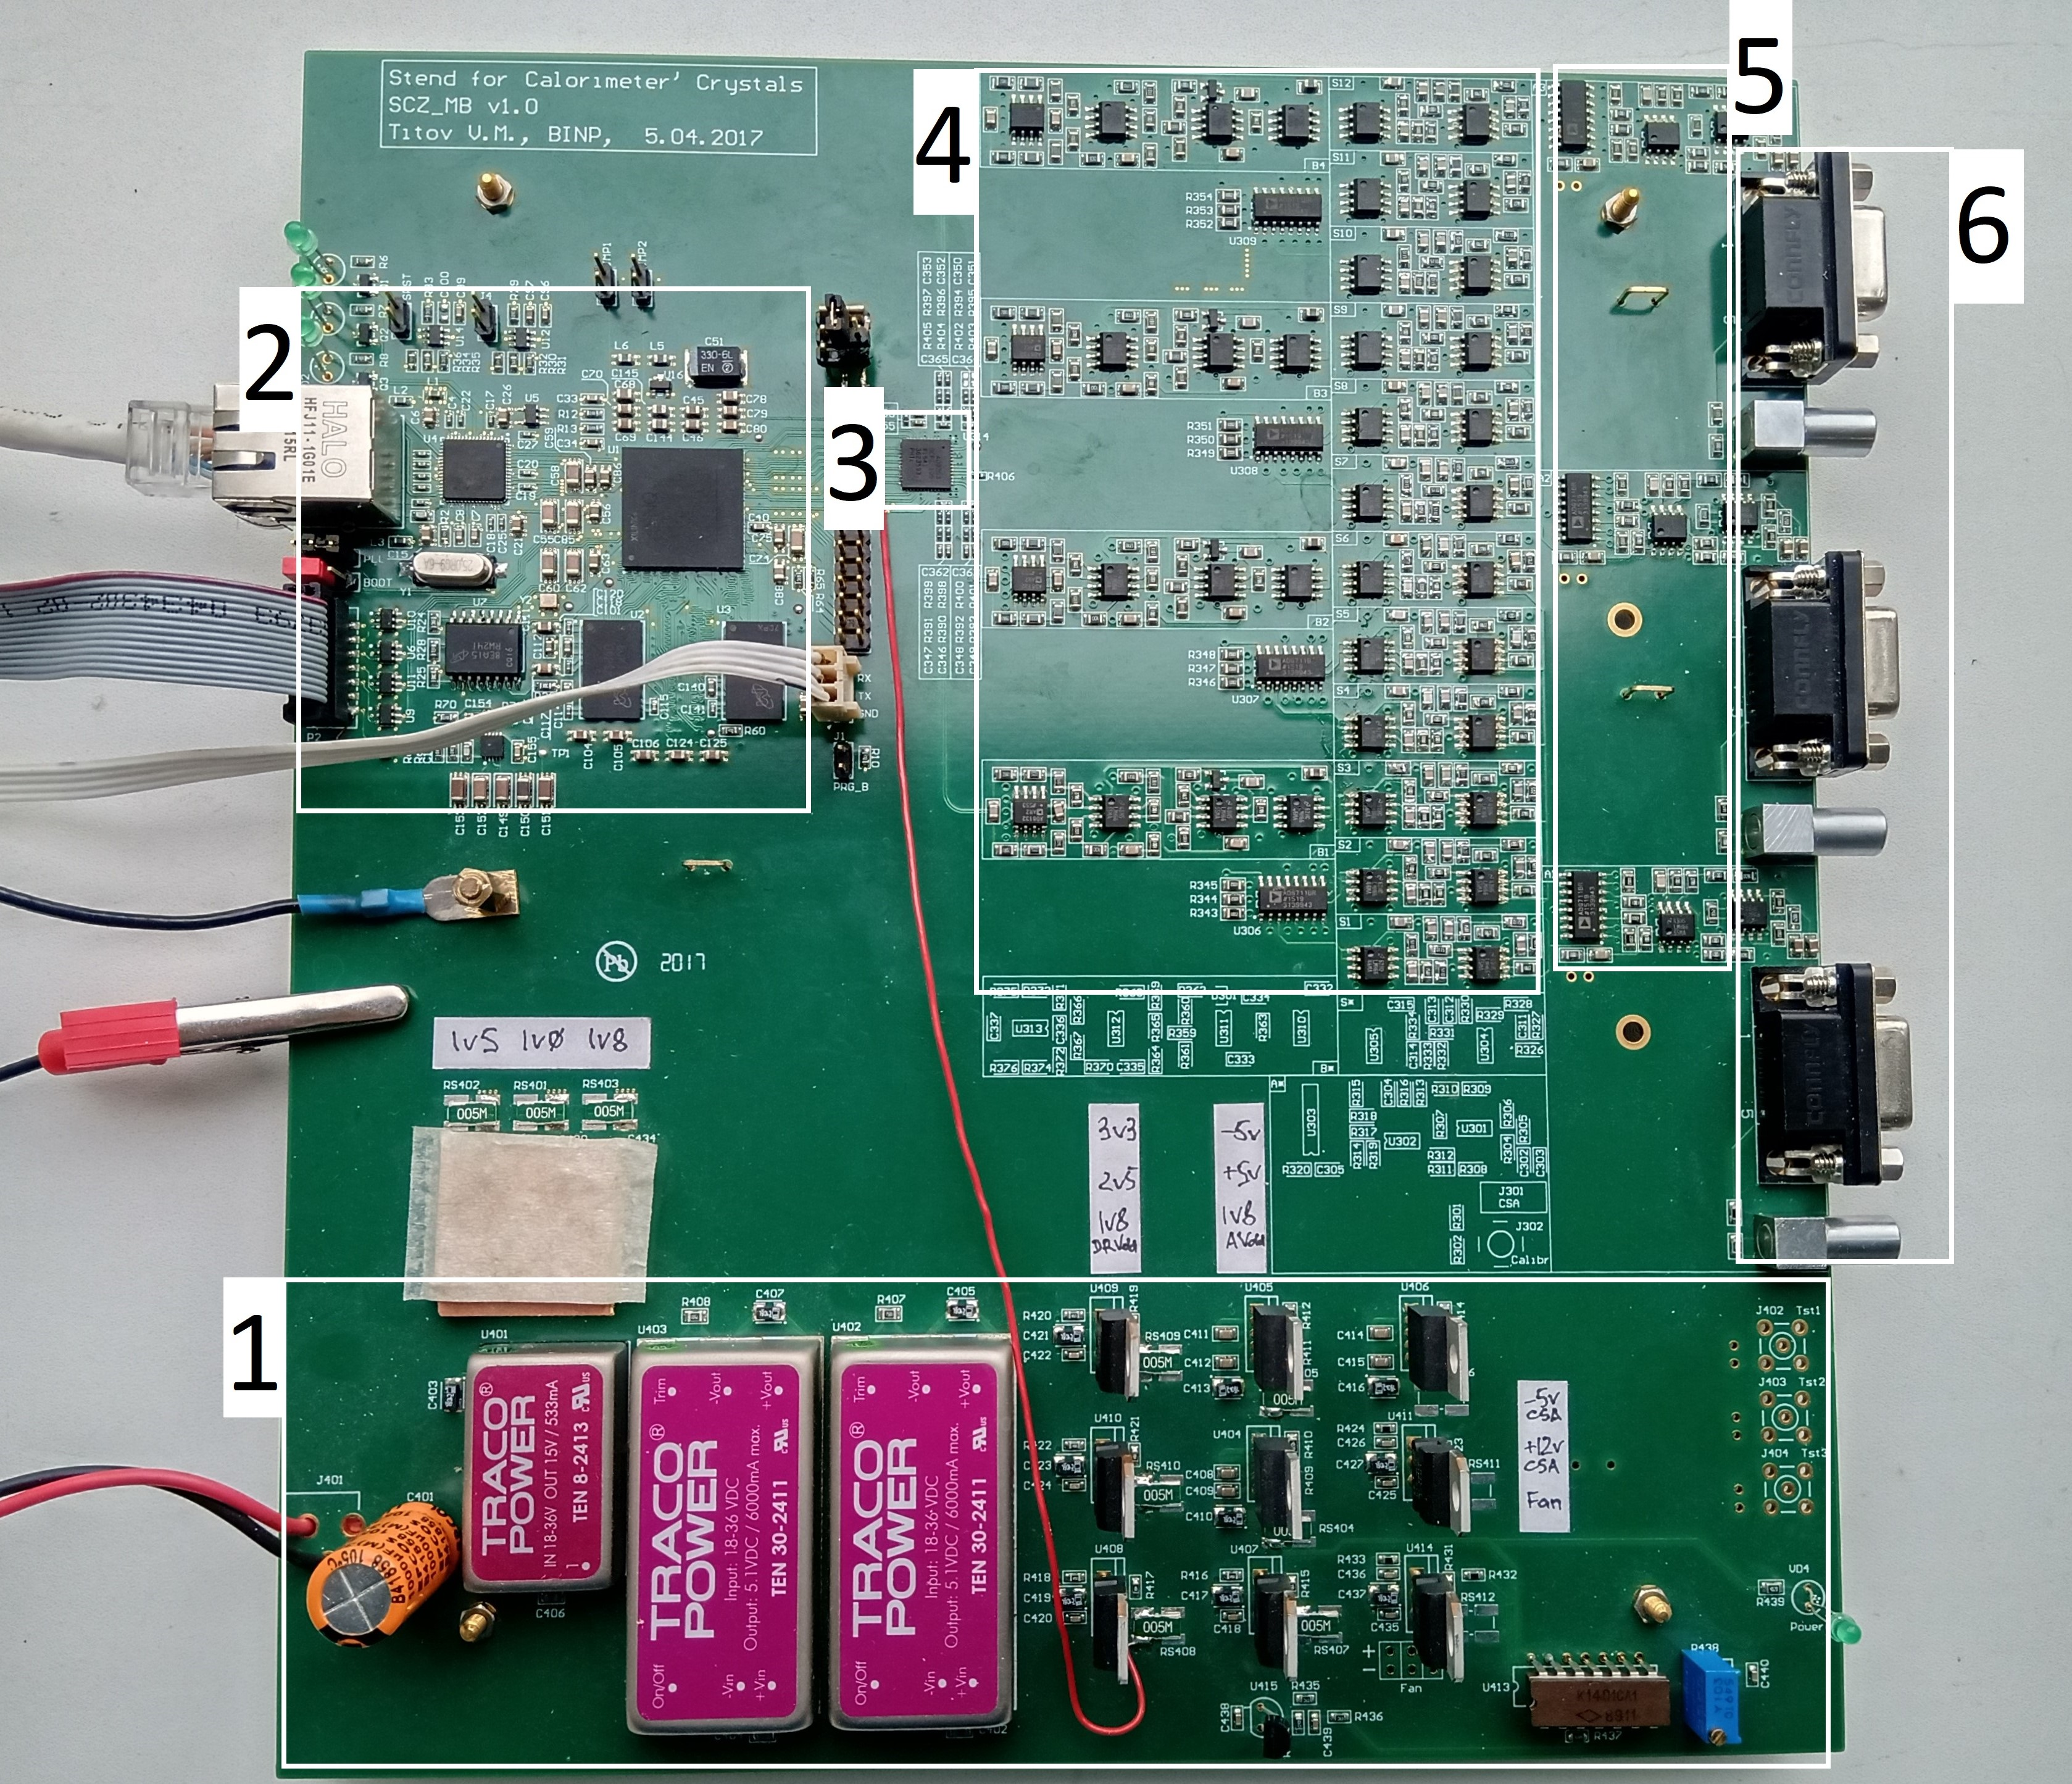
\includegraphics[width=1\linewidth]{board.jpg}
    \caption{Фотография стенда: 1 - блок питаний; 2 - СнК ZYNQ-7000 с необходимой периферией; 3 - АЦП; 4 - формирователи основного и вспомогательных сигналов; 5 - усилители сигналов; 6 - входные разъемы}
    \label{fig:board}
\end{figure}
Далее будут рассмотрены подробнее особенности устройства некоторых частей описанной системы.\par
\textbf{Основной канал}\par
Основной канал имеет 2 набора формирователей с различными временами формирования: 0.1, 0.2, 0.5 и 1, 2, 5 мкс соответственно. Данные временные значения формирователей подобраны на основе анализа свойств сцинтилляционных кристаллов, а также имеющегося опыта работы с ними. Выбранные значения позволяют обеспечить корректную работу с широким набором кристаллов: от имеющих сравнительно малое время высвечивания до обладающих длительным.\par
После каждого формирователя установлены электронные ключи, с помощью которых можно подключить выход одной секции из набора через буфер ко входу АЦП. Таким образом, на основном канале имеется возможность подключить одновременно 2 формирователя из диапазона 0.1 - 0.5 и 1 - 5 мкс соответственно. Оцифрованные данные непрерывно записываются в кольцевой буфер, откуда они могут быть выгружены для обработки и сохранения при поступлении сигнала о полезном событии от триггерной системы.\par
\textbf{Вспомогательные каналы}\par
Вспомогательные каналы служат источниками дополнительных сигналов, необходимых для правильной работы триггерной системы. Устройство вспомогательных каналов практически аналогично основному. Отличия:\par
\begin{itemize}
    \item каждый из них содержит только по одному набору формирователей с тремя секциями с временами 0.1, 0.2, и 0.5 мкс;
    \item к аналогово-цифровому преобразователю может быть подключен выход только одной секции формирования канала.
\end{itemize}\par
\textbf{Триггерная система}\par
Триггерная система выполняет задачу формирования сигнала, означающего возникновение полезного события, при котором данные из кольцевого буфера необходимо выгрузить для последующей обработки. Система может работать в двух режимах: принудительный старт и срабатывание по порогу. В первом случае триггерная система вырабатывает сигнал при получении команды от оператора. Во втором случае триггер срабатывает при превышении текущими цифровыми значениями основного и/или некоторых вспомогательных каналов заданных оператором порогов.
